\begin{figure}[t]
    \centering
    \begin{minipage}{0.2\textwidth}
        \centering
        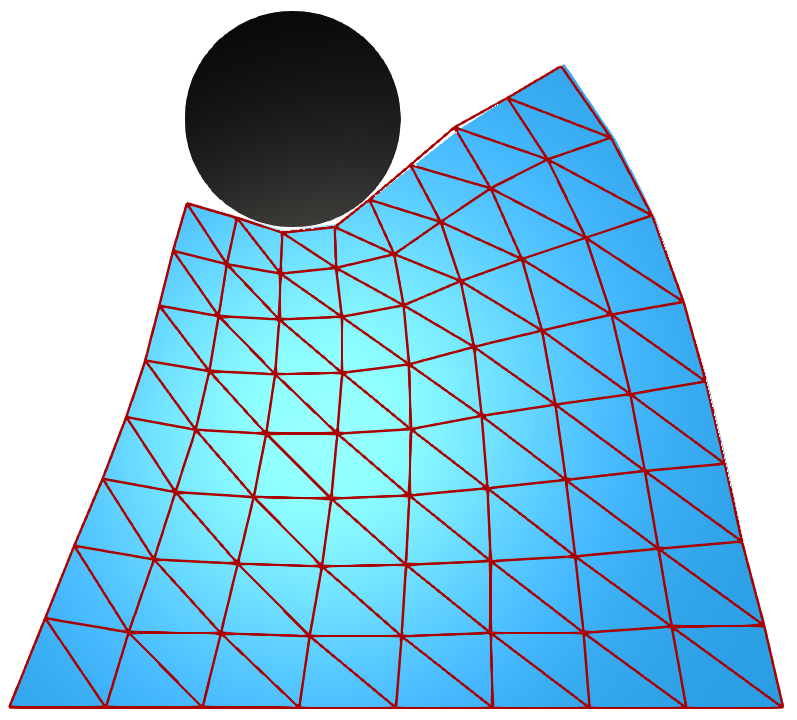
\includegraphics[width=\textwidth]{figures/task_overview_data/db.png}
    \end{minipage}
    \hspace{1mm}
    \begin{minipage}{0.29\textwidth}
        \centering
        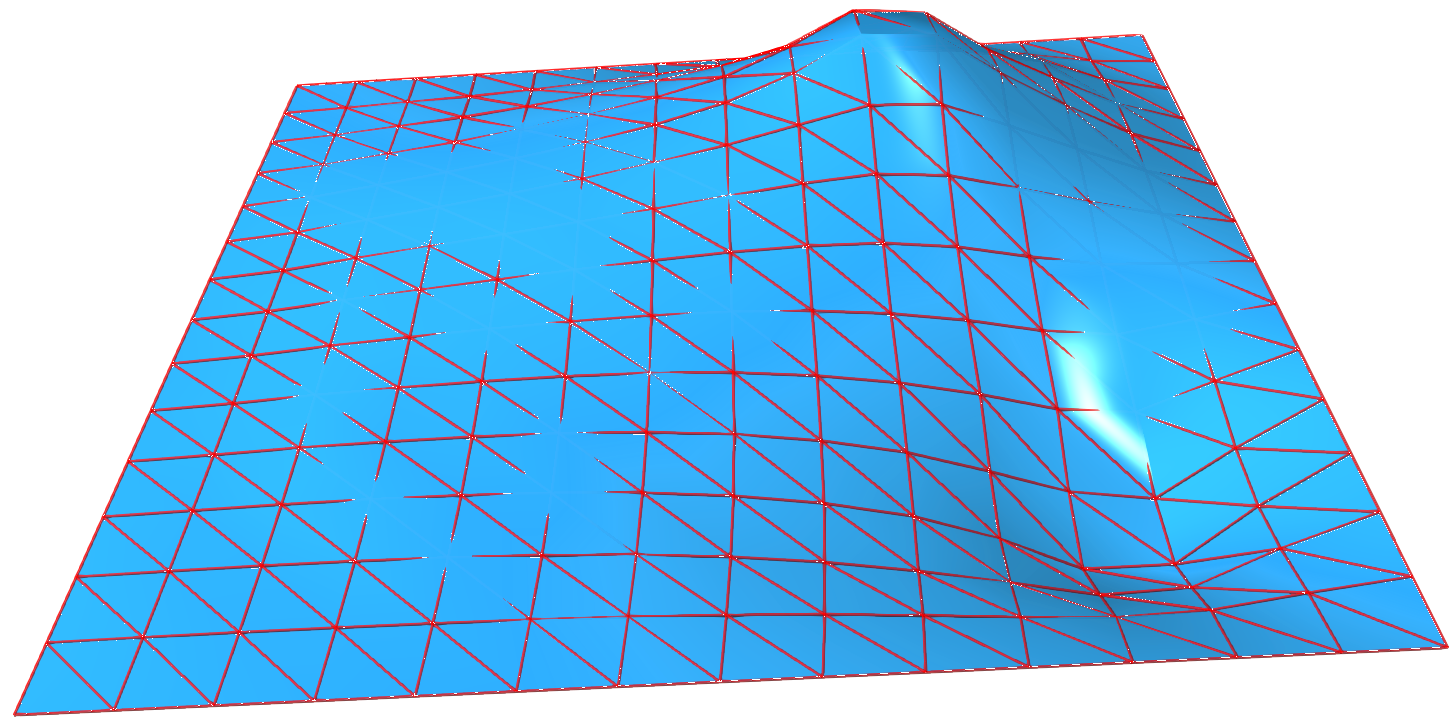
\includegraphics[width=\textwidth]{figures/task_overview_data/sd.png}
    \end{minipage}
    \begin{minipage}{0.48\textwidth}
        \centering
        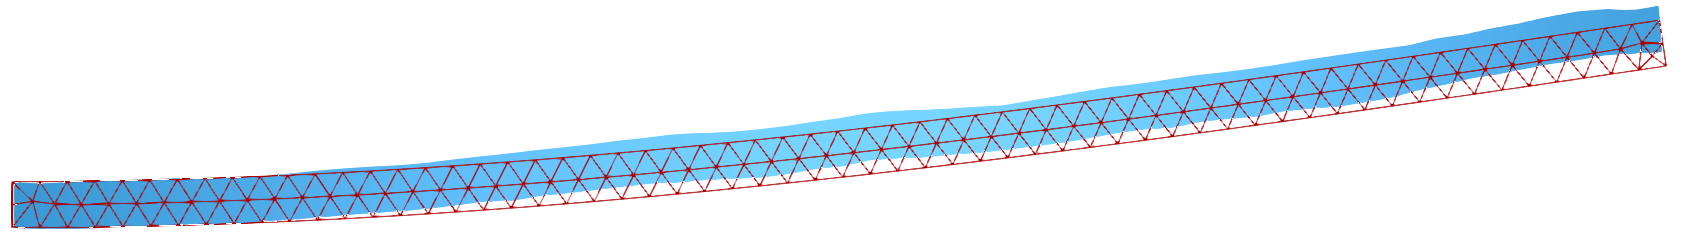
\includegraphics[width=\textwidth]{figures/task_overview_data/bbv.png}
    \end{minipage}%
\vspace{0.05mm}

    \begin{minipage}{0.2\textwidth}
        \centering
        {\small \texttt{Deforming Block}}
    \end{minipage}
    \begin{minipage}{0.29\textwidth}
        \centering
        {\small \texttt{Sheet Deformation}}
    \end{minipage}
    \begin{minipage}{0.48\textwidth}
        \centering
        {\small \texttt{Bending Beam}}
    \end{minipage}%
\vspace{-5mm}

    \begin{minipage}{\textwidth}
        \centering
        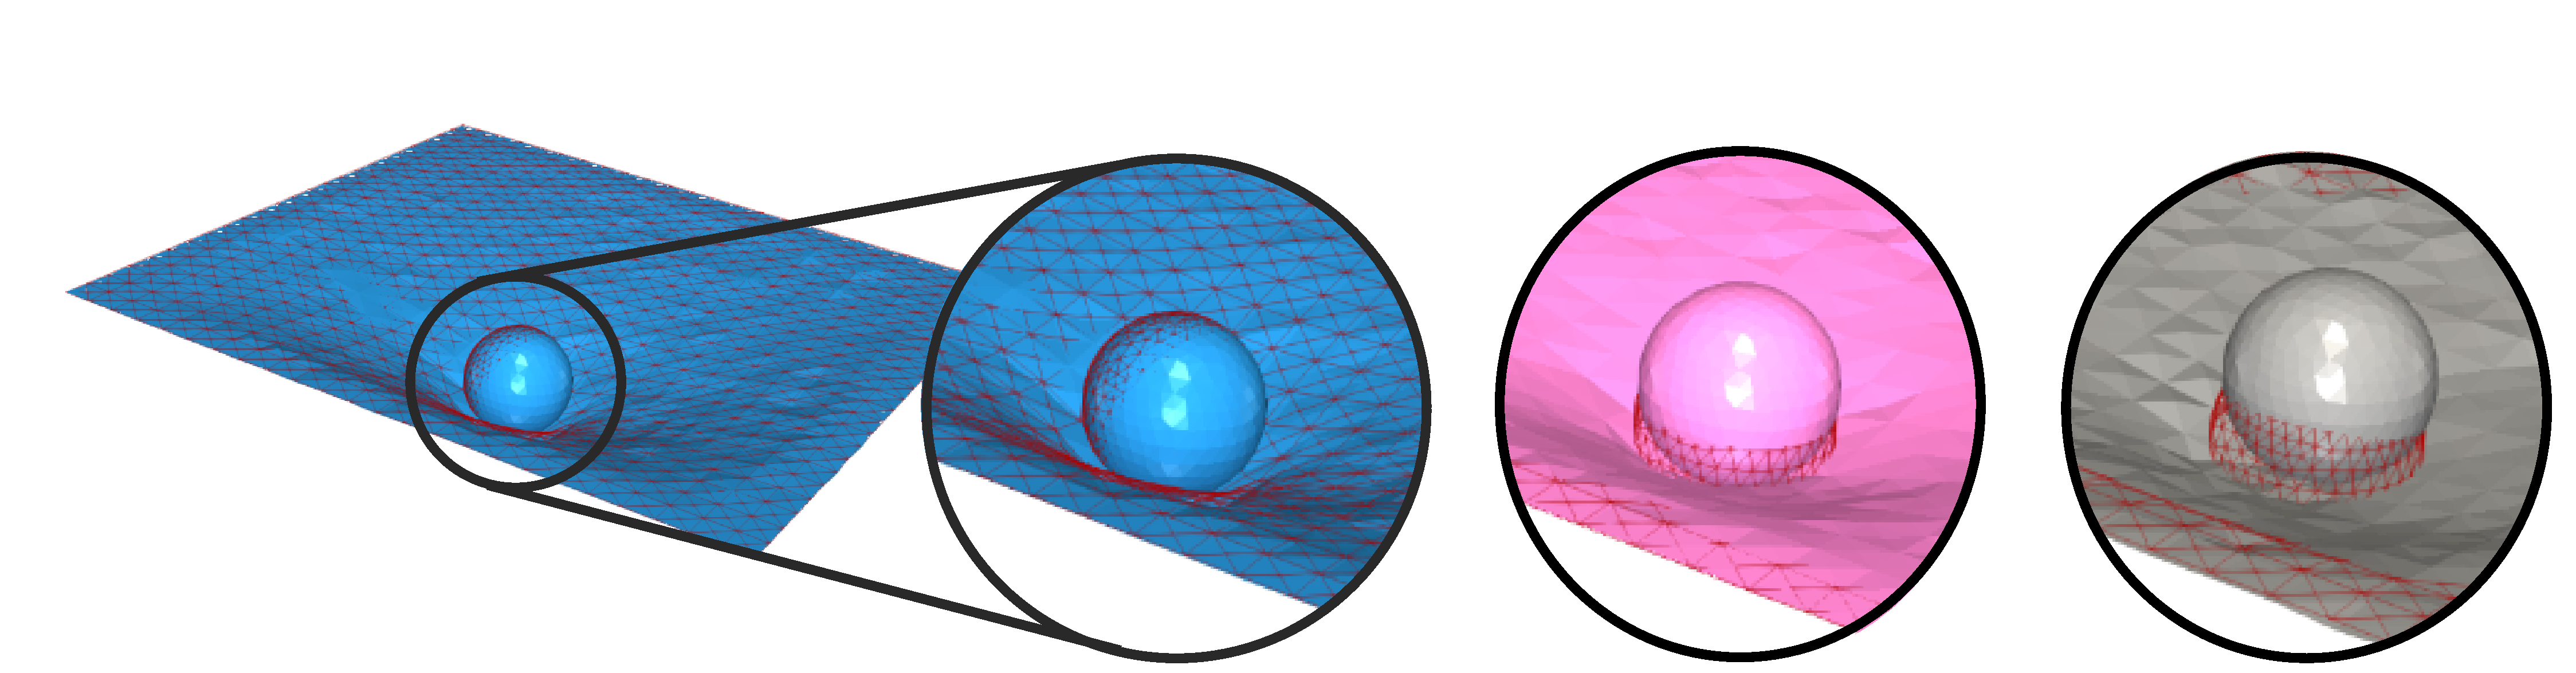
\includegraphics[width=\textwidth, trim={50 0 0 0}, clip]{figures/task_overview_data/task_overview.pdf}
    \end{minipage}

    % \begin{minipage}{0.325\textwidth}
    %     \centering
    %     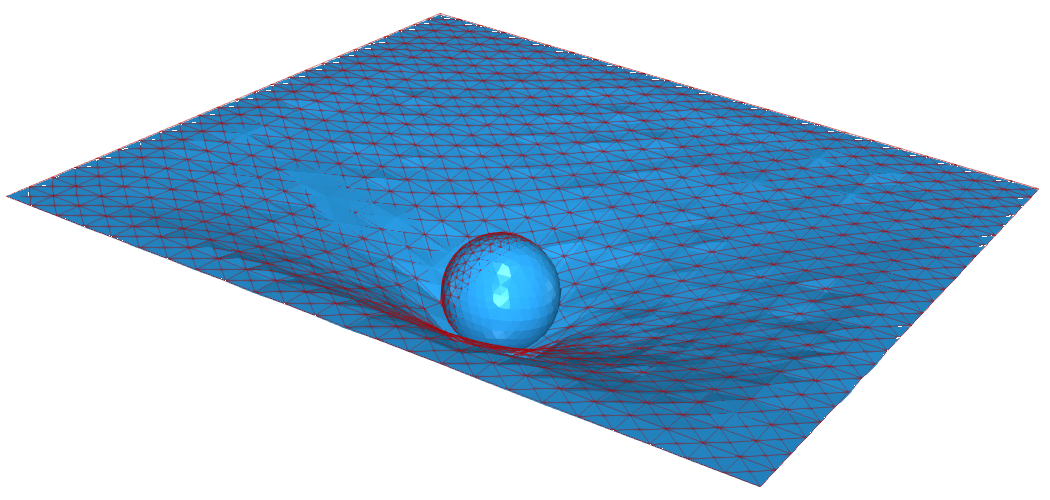
\includegraphics[width=\textwidth]{figures/task_overview_data/trampoline_peach.png}
    % \end{minipage}
    % \begin{minipage}{0.325\textwidth}
    %     \centering
    %     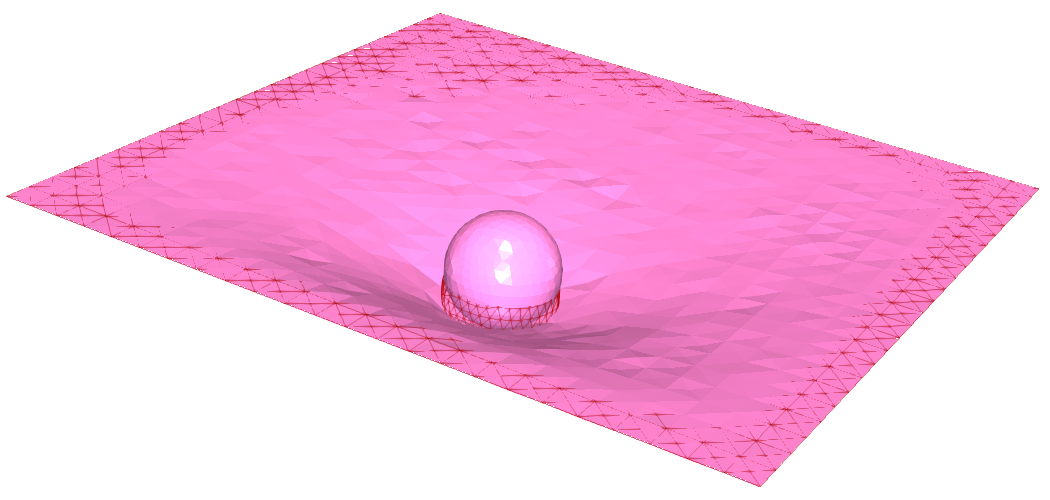
\includegraphics[width=\textwidth]{figures/task_overview_data/trampoline_pstnet.png}
    % \end{minipage}
    % \begin{minipage}{0.325\textwidth}
    %     \centering
    %     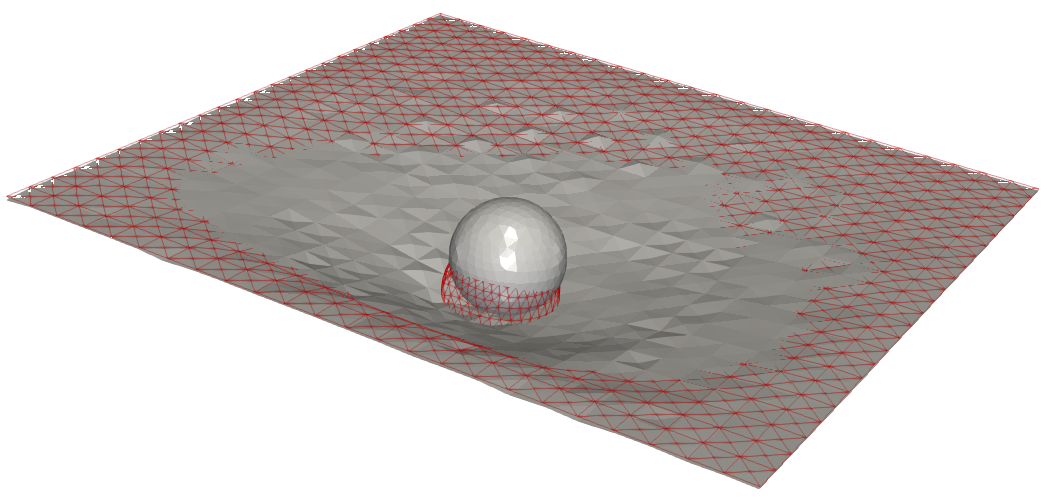
\includegraphics[width=\textwidth]{figures/task_overview_data/trampoline_dummy.png}
    % \end{minipage}%
    % \vspace{0.05mm}
    
    \begin{minipage}{0.3\textwidth}
        \centering
        {\small \texttt{Trampoline }}
    \end{minipage}
    \begin{minipage}{0.2\textwidth}
        \centering
        {\small \hspace{0.6cm} \textit{PEACH}}
    \end{minipage}
    \begin{minipage}{0.23\textwidth}
        \centering
        {\small \hspace{0.8cm}\textit{PSTNet Encoder}}
    \end{minipage}
    \begin{minipage}{0.23\textwidth}
        \centering
        {\small \hspace{0.5cm} \textit{No Context}}
    \end{minipage}
    


\caption{
    Overview of the four simulation scenes.
    The environments cover a range of deformable object types and material models, from purely elastic to viscoelastic constitutive behaviors, with varying material properties across tasks.
    Qualitative predictions of \gls{peach} and selected baselines are shown in \textcolor{blue}{blue}, \textcolor{TabPink}{pink}, and \textcolor{gray}{gray}, respectively, with ground-truth meshes overlaid in \textcolor{red}{red}.
}
\vspace{-0.6cm}
\label{fig:task_overview}
\end{figure}
